\chapter{Objektidentifiering}
För att få en mer användarvänlig robothand har möjligheten till objektidentfiering behandlats. Genom att handen identifierar objekten den greppar kan den själv justera det maximalt tillåtna trycket från förinställda värden och förhindra risken att objekten utsätts för ett övertryck. Efterssom objektidentifieringen automatisera denna del slipper användaren reglera trycket vilket ger ett mycket mer intuitivt och lättanvändligt system. Bild \ref{fig:objektidentifiering1} illustrerar hur objektidentifieringen är upplagd.

\begin{figure}[H]
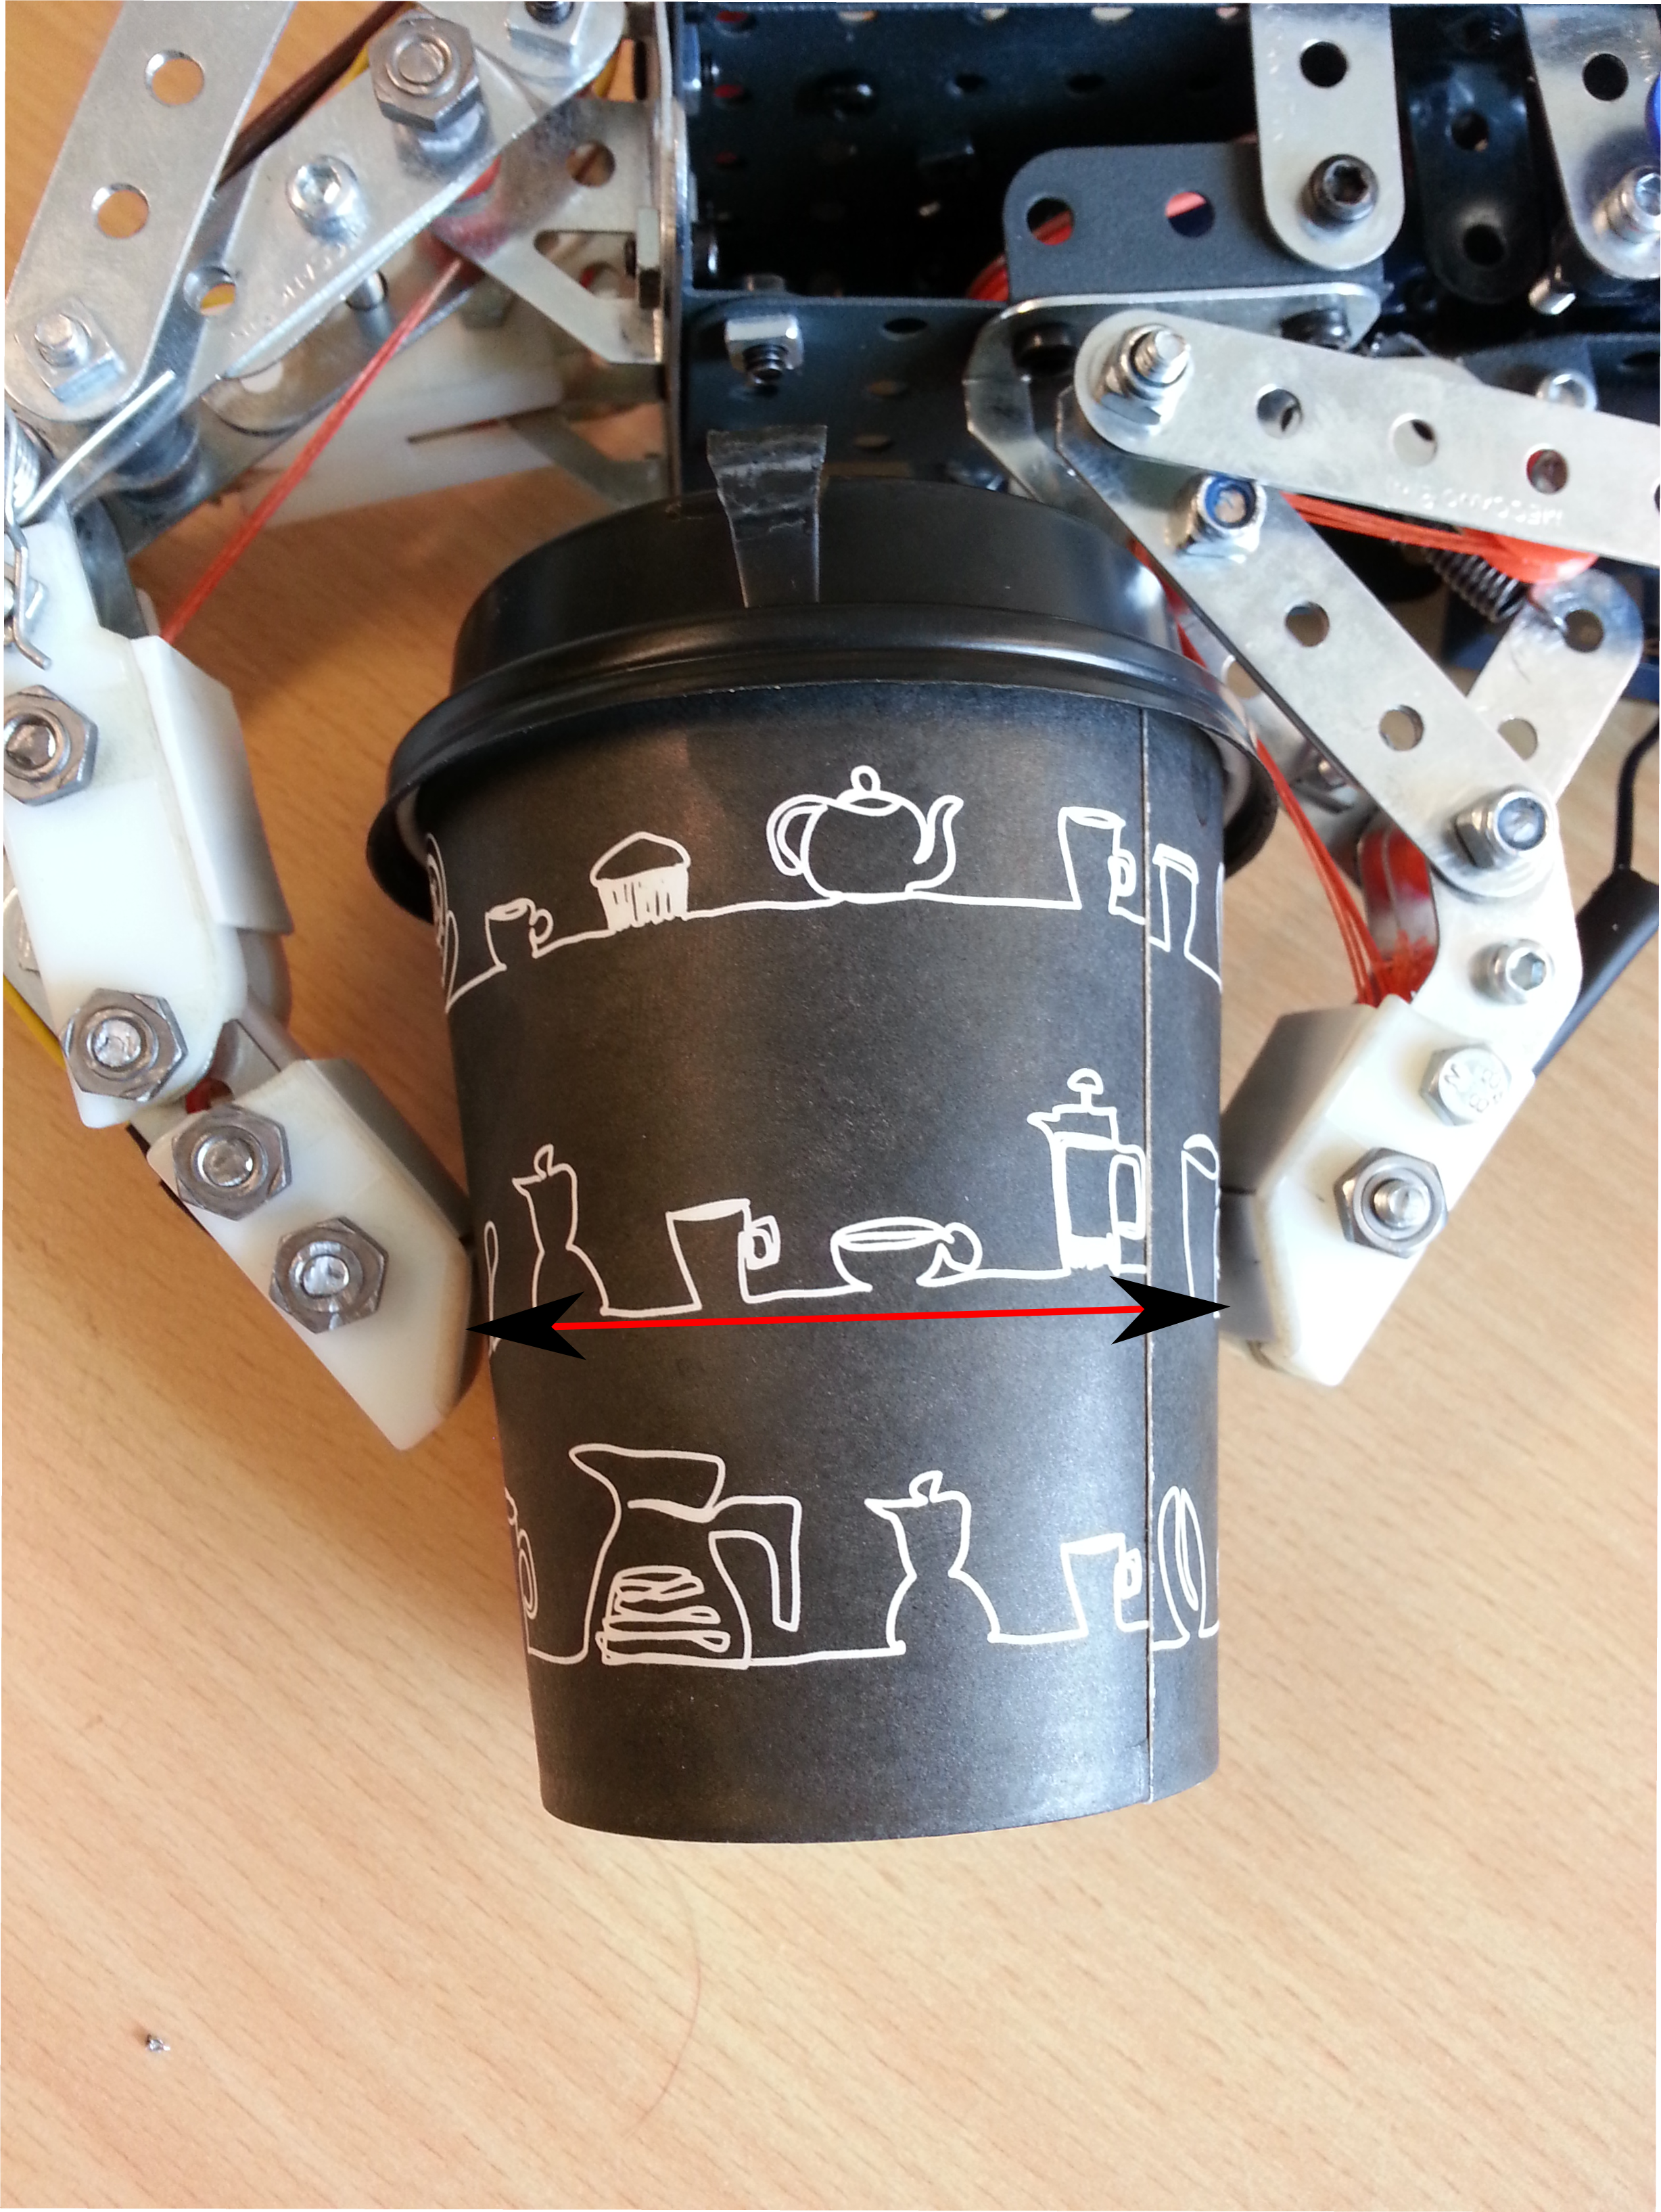
\includegraphics{img/obj_dist}
\caption{Identifiering av objekt}
\label{fig:objektid}
\end{figure}



Objektidentifieringen bygger på att handen beräknar distansen mellan fingertopparna där trycksensorerna sitter och därigenom får information om vilka objekt som greppas för att sedan ta beslut om hur hårt tryck som är tillåtet. För att möjliggöra detta har en mattematiskmodell över handens rörelse tagits fram, se \ref{servoberakningar}. Modellen baseras på servovinklarna ($\varphi_1$,$\varphi_2$,$\varphi_3$,$\varphi_4$) som är de servolägen som styr de fyra lederna i tummen och pekfingret. Modellen kopplar de önskade servolägerna till koordinater för ändpunkter på fingrarna och därigenom avståndet mellan punkterna. Modellen är 2-dimensionell och baseras på att tumme och pekfinger rör sig i samma plan. \

\begin{figure}[H]
\includegraphics[width=\textwidth]{img/servo/objektidentifiering}
\caption{Schematisk bild över objektidentifiering}
\label{fig:objektidentifiering1}
\end{figure}

Objektidentifieringen har ett genomsnittligt fel på 20\%. Felet varierar beroende på i vilket område fingrarns befinner sig i. Arbetsområdet rekonmenderas att ligga mellan 40-100 mm där en upplösning på 15 mm erhålles. Figur \ref{fig:verk_berak} jämför uppmätta värden med de värden framtagna med hjälp av den mattematiska modellen. För att få en ökad precision rekomenderas att de felkällor som tas upp i \ref{felkallor} åtgärdas. Figur \ref{fig:objektidentifiering2} visualiserar handens rörelse med hjälp av den mattematiska modellen.

\begin{figure}[H]
\includegraphics[width=0.8\textwidth]{img/obj_id_matlab2}
\caption{plot över det uppmätta avstånden jämfört med det uträknade}
\label{fig:verk_berak}
\end{figure}

\begin{figure}[H]
\includegraphics[width=\textwidth]{img/obj_id_matlab}
\caption{plot över fingrets rörelse från den matematiska modellen}
\label{fig:objektidentifiering2}
\end{figure}


\subsubsection{Felkällor}
\label{felkallor}
Objektidentifieringen inehåller främst två felkällor som bidrar till en minskad precision. En av felkällorna är att modellen är baserat på önskade servolägen, dvs de lägen som specificerats av användaren. Om servomotorerna möter på motstånd som förhindrar rörelse till önskat läge kommer det faktiska avståndet och det avstånd beräknat genom modellen att skillja vilket bidrar till ett fel. Bild \ref{fig:objident1}-\ref{fig:objident2} illutrerar en situation då detta fel inträffar.

\begin{figure}[H]

        \begin{subfigure}[b]{0.5\textwidth}
                \centering
                \includegraphics{img/grepp}
                \caption{Faktiskt servoläge}
                \label{fig:objident1}
        \end{subfigure}%
       ~
        \begin{subfigure}[b]{0.5\textwidth}

                \includegraphics{img/grepp_verk}
                \caption{Önskat servoläge}
                \label{fig:objident2}
        \end{subfigure}

\end{figure}

För att lösa detta problem behöver systemet få information om handens faktiska läge. Detta kan åstadkommas genom att ansluta vinkelgivare till fingrets leder alternativt till servomotorerna. \

En annan stor felkälla är att handens konstruktion bidrar med låg precision, pga det mekaniska glappet. Mekanots låga toleranser gör att ett givet servoläge kan innebära många olika positioner. Felkällans magnitud ökar fort med ett ökat antal leder. För att öka precisionen behövs konstruktionen ändras för att exkludera det mekaniska glappet.
